\documentclass{beamer}
\usepackage{pagegard}% test for table
\usepackage{xspace}


% \renewcommand*{\theauthor}{Ayoub EL MHAMDI}
\renewcommand*{\professeur}{Amal KCHIBAL}
\newcommand*{\flag}{-}

\begin{document}


% Title page frame
% \maketitle
\placelogotrue

% \begin{frame}{OBJECTIF}
%     ii
% \end{frame}
% {\placelogofalse
% \begin{frame}{PLAN}
%   \setbeamertemplate{section in toc}[sections numbered]
%     \textbf{
%       \tableofcontents%[hideallsubsections]
%     }
% \end{frame}
% }
% \section{INTRODUCTION}
% \begin{frame}{INTRODUCTION}
%     contenu
%     Some references to showcase\cite{knuth92,ConcreteMath,Simpson,Er01,greenwade93}
% \end{frame}

% \section{HISTORIQUE}
% \begin{frame}{test3}
%     \begin{enumerate}[<+-|alert@+>]
%         \item
%         Effects that control
%
%         \item
%         when text is displayed
%
%         \item
%         are specified with <> and a list of slides.
%     \end{enumerate}
%
%     \begin{block}{new theme}<1>
%         kkk
%     \end{block}
%
%     \begin{theorem}<2>
%         This theorem is only visible on slide number 2.
%     \end{theorem}
% \end{frame}
% \section*{REF1}
%
% \section{CONCLUSION}
% \begin{frame}[allowframebreaks]{Conclusion}
%     for hhh
% \end{frame}
%
% \begin{frame}[allowframebreaks]{References}
%     \bibliography{demo}
%     \bibliographystyle{abbrv}
% \end{frame}
%
% {\placelogofalse
% \begin{frame}[standout]
%     Merci de Votre Aimable Attention
% \end{frame} 
% }

\section{HISTORIQUE}
\subsection{1950}
\subsection{1970}
\subsection{1980}

% 
\section{Historique}
\subsection{1950}
\subsection{1970}
\subsection{1980}
{\placelogotrue
\begin{frame}{Historique}
    \begin{enumerate}[$\blacksquare$]
        \item 1950
            \only<1>{
            \begin{exampleblock}{Naissance du mot}
                le $ mot $ de IA est née dans les années 1950 avec l'objectif de faire
                produire des tâches humaines par des machines mimant l'activité du
                cerveau.
                %que ce soit par des algorithmes des
                %classification/reseux des neurons artificiels
                % image de alan torine dans reunis
            \end{exampleblock}
            }

        \item 1970
            \only<2>{
            \begin{exampleblock} {Création des algorithmes}
                les scientifique ont pris fin à création de tous les algorithmes
                d'intelligence artificiels, mais la puisance des ordinateurs sont très
                faibles
            \end{exampleblock}
            }

        \item 1980
            \only<3>{ \begin{exampleblock}{Mycin}
                le développement du premier applications qui utilise le IA dans le
                domaine de medcine, qui capable de reproduire les mécanismes cognitifs
                d'un expert, Les plus célèbres, Mycin (identification d'infections
                bactériennes) s'appuient sur l'ensemble des connaissances médicales
                dans un domaine donné et une formalisation des raisonnements des
                spécialistes qui lient ces connaissances entre elles pour aboutir à un
                diagnostic.
            \end{exampleblock}
            }

        \item  à partir de 1980
            \only<4>{
            \begin{exampleblock}{Réseaux des neurones artificielle}
                développement des réseaux de neurones artificiels, grâce à l'augmentation
                de puissance des ordinateurs et à l'accumulation des gigantesques quantités
                de données(big data).
            \end{exampleblock}
            }

        \item récent\only<5>{
            \begin{exampleblock}{Google}
                Google AI mis au point une IA qui prédit le cancer du poumon avec
                $94,4~\%$ de réussite. Ces procédures permettent aussi d'éviter des
                tests invasifs comme des biopsies. L'IA apporte également une aide à
                la prescription, par exemple en détectant automatiquement un risque
                d'allergie ou d'interaction médicamenteuse.
            \end{exampleblock}
            }
            \vspace{80mm}
    \end{enumerate}
\end{frame}
}

\section{Introduction}
\subsection{\mybox Définition}
\subsection{\mybox Machine Learninig}
\subsection{\mybox Deep Learning}
\subsection{\mybox Des applications}
\subsection{\mybox Experts  vs IA}

\begin{frame}{Introduction}
    \begin{enumerate}[<+-|alert@+>]
        \myitem
        L'intelligence artificielle est partout, mais elle trouve plus 
        particulièrement des applications intéressantes dans le domaine
        de la santé.

        \myitem
        Les données médicales constituent une ressource inestimable pour prédire des maladies,
        diagnostiquer une pathologie ou améliorer le suivi des patients.

        \myitem
        L'\textbf{IA} est capable de poser un diagnostic fiable ou de lever des soupçons sur des
        pathologies.\mybox
    \end{enumerate}
\end{frame}




\begin{frame}{Définition}
    \begin{itemize}[<+-|alert@+>]
        \myitem
            ``L'intelligence artificielle'' \textbf{IA} est l'ensemble des théories
            et des techniques mises en œuvre en vue de réaliser des
            machines capables de simuler ``l'intelligence humaine''

        \myitem
            Les algorithmes de \textbf{IA} est basé sur  l'injections des
            milliards de données dans un programme d'apprentissage,

        \myitem
        dans le cas des algorithmes du médecine, on apprend à ``reconnaître''
        les signes de la maladie.\mybox
    \end{itemize}
    \only<1->{
        \centering
        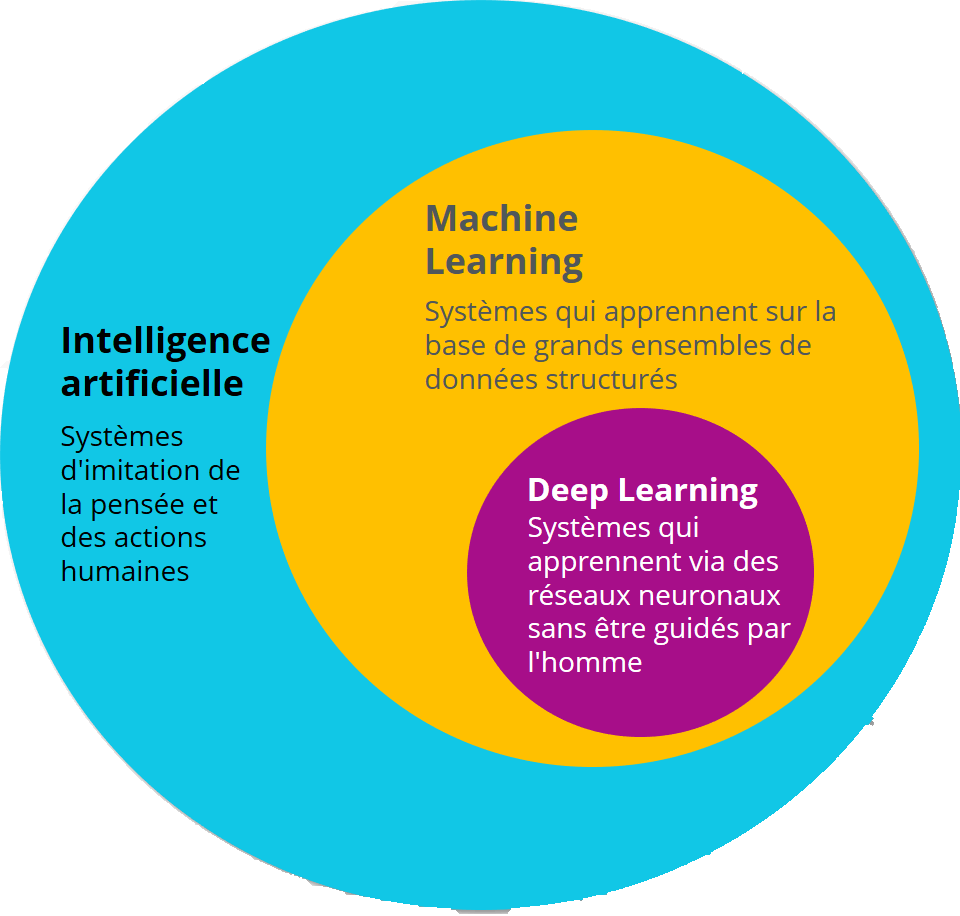
\includegraphics[height=0.3\textwidth,width=0.3\textwidth]{ai1a.png}
    }

\end{frame}

\begin{frame}{Machine Learninig}
    \begin{itemize}[<+-|alert@+>]
        \myitem
        ``Machine learninig'' apprentissage automatique, une méthode fondée sur
        la représentation mathématique et informatique de neurones
        biologiques, selon des modalités plus ou moins complexes.

        \myitem
        La force de cette technique est que l'algorithme apprend la
        tâche qui lui a été assignée par ``essais et erreurs''.\mybox
    \end{itemize}

    \only<1-2>{
        % \vspace{0mm}
        \centering
        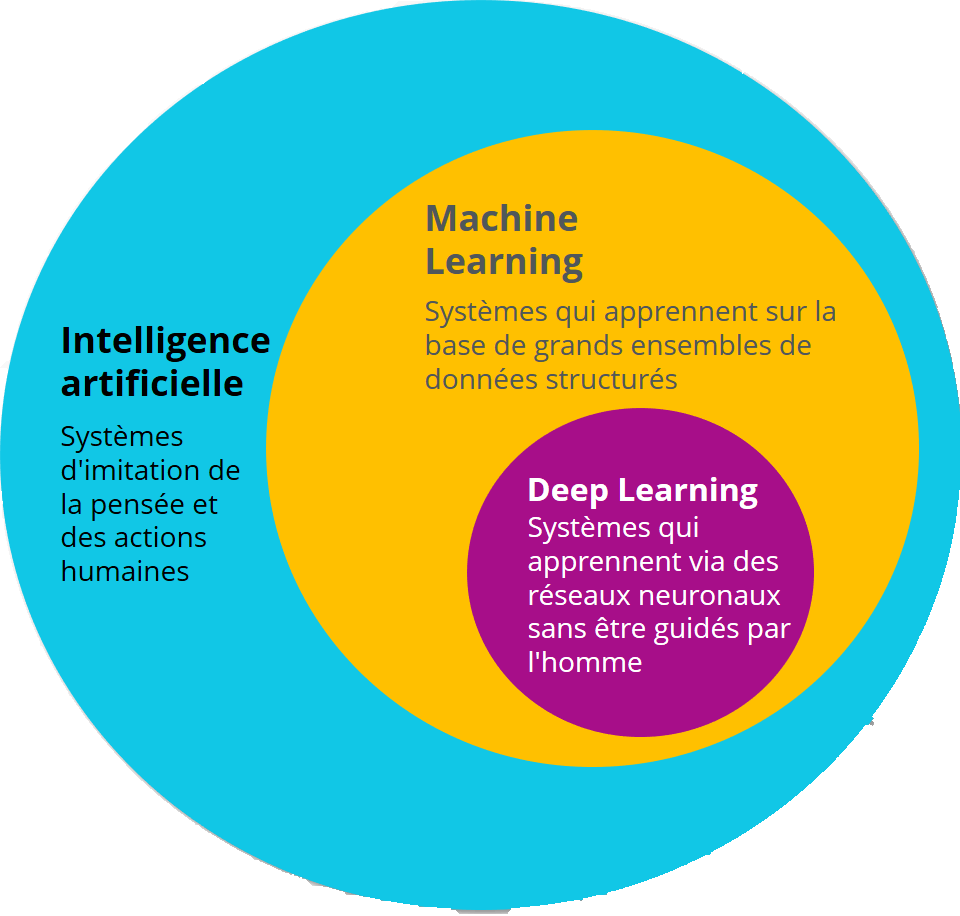
\includegraphics[height=0.4\textwidth,width=0.4\textwidth]{ai1a.png}
    }
    \vspace{80mm}

\end{frame}

\begin{frame}{Deep Learning}
    Utilisation des algorithmes d'intelligence artificielle pour permettre
    en quelque sorte aux ordinateurs d'apprendre par eux-mêmes On
    appelle cela l'apprentissage profond ou ``deep learning'' en anglais''.\mybox
    \\
    \bigskip
    \bigskip
    \centering
    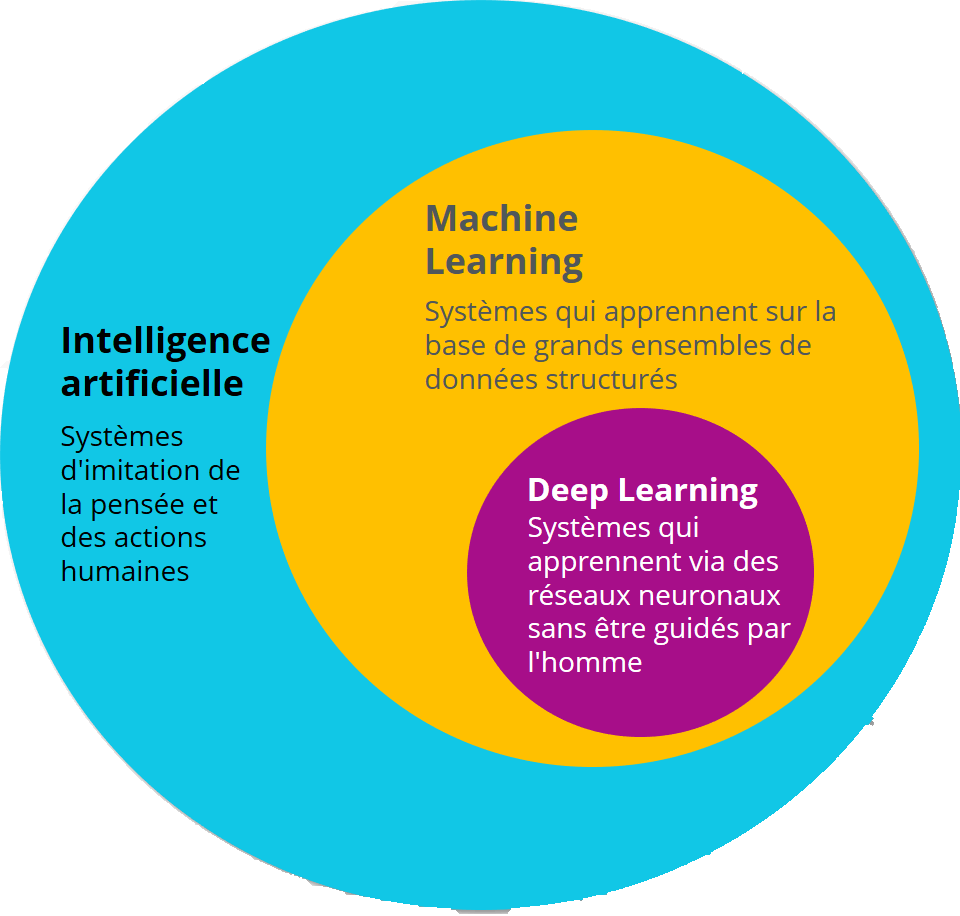
\includegraphics[height=0.3\textwidth,width=0.3\textwidth]{ai1a.png}
\end{frame}

\begin{frame}{Des applications}
    \begin{enumerate}[<+-|alert@+>]
        \myitem
        l'application de \textbf{IA} en traitement d'images, par exemple pour repérer de
        possibles mélanomes sur les photos de peau, ou bien pour dépister des
        rétinopathies diabétiques sur des images de rétines. Leur mise au point
        nécessite de grands échantillons d'apprentissage.
        \myitem
        en prend plus de 50 000 images dans le cas des mélanomes, et 128 000
        dans celui des rétinopathies, ont été nécessaires pour entraîner
        l'algorithme à identifier les signes de pathologies. Pour chacune
        de ces images on lui indique si elle présente ou non des signes
        pathologiques.
        \myitem
        A la fin de l'apprentissage, l'algorithme arrive à
        reconnaître avec une excellente performance de nouvelles images
            présentant une anomalie. \mybox
    \end{enumerate}
\end{frame}


\begin{frame}{Experts  vs IA}
    \begin{enumerate}[]
        \item \only<1->{
            \begin{exampleblock}{Les experts:}
                les procédures interventionnelles demandent une dextérité
                manuelle et un sens commun pour s'adapter à des situations changeantes.
            \end{exampleblock}
            }

        \item \only<2>{
            \begin{exampleblock} {IA:}
                Le travail des médecins radiologistes comprend de nombreuses tâches,
                dont les plus rapides comme la détection d'une anomalie ou les plus
                répétitives comme les mesures se prêtent bien à l'automatisation.\mybox
            \end{exampleblock}
            }
            \vspace{80mm}
    \end{enumerate}
\end{frame}


\end{document}
